% ------------------------------------------------------------------------------
% Formatvorlage für Masterarbeiten an der Ohm-Hochschule Nürnberg
% ------------------------------------------------------------------------------
%   erstellt von Stefan Macke, 24.04.2009
%   http://blog.stefan-macke.de

% Dokumentenkopf ---------------------------------------------------------------
%   Diese Vorlage basiert auf "scrreprt" aus dem koma-script.
% ------------------------------------------------------------------------------
\documentclass[
    11pt, % Schriftgröße
    DIV10,
    english, % für Umlaute, Silbentrennung etc.
    a4paper, % Papierformat
    oneside, % einseitiges Dokument
    titlepage, % es wird eine Titelseite verwendet
    parskip=half, % Abstand zwischen Absätzen (halbe Zeile)
    headings=normal, % Größe der Überschriften verkleinern
    listof=totoc, % Verzeichnisse im Inhaltsverzeichnis aufführen
    bibliography=totoc, % Literaturverzeichnis im Inhaltsverzeichnis aufführen
    index=totoc, % Index im Inhaltsverzeichnis aufführen
    captions=tableheading, % Beschriftung von Tabellen unterhalb ausgeben
    final % Status des Dokuments (final/draft)
]{scrreprt}

% Meta-Informationen -----------------------------------------------------------
%   Informationen über das Dokument, wie z.B. Titel, Autor, Matrikelnr. etc
%   werden in der Datei Meta.tex definiert und können danach global
%   verwendet werden.
% ------------------------------------------------------------------------------
% Meta-Informationen -----------------------------------------------------------
%   Definition von globalen Parametern, die im gesamten Dokument verwendet
%   werden können (z.B auf dem Deckblatt etc.).
%
%   ACHTUNG: Wenn die Texte Umlaute oder ein Esszet enthalten, muss der folgende
%            Befehl bereits an dieser Stelle aktiviert werden:
%            \usepackage[latin1]{inputenc}
% ------------------------------------------------------------------------------
\newcommand{\titel}{Titel der Masterarbeit}
\newcommand{\untertitel}{und hier kommt der Untertitel}
\newcommand{\art}{Masterarbeit}
\newcommand{\fachgebiet}{Software-Engineering}
\newcommand{\autor}{Hans Meier}
\newcommand{\studienbereich}{Software-Engineering}
\newcommand{\matrikelnr}{12 34 56}
\newcommand{\erstgutachter}{Prof. Dr. Werner Berentzen}
\newcommand{\zweitgutachter}{Dipl.-Inf. Lukas Podolski}
\newcommand{\jahr}{2009}
\newcommand{\ort}{Berlin}
\newcommand{\logo}{LogoOhmHochschule.jpg}


% benötigte Packages -----------------------------------------------------------
%   LaTeX-Packages, die benötigt werden, sind in die Datei Packages.tex
%   "ausgelagert", um diese Vorlage möglichst übersichtlich zu halten.
% ------------------------------------------------------------------------------
% Anpassung des Seitenlayouts --------------------------------------------------
%   siehe Seitenstil.tex
% ------------------------------------------------------------------------------
\usepackage[
    automark, % Kapitelangaben in Kopfzeile automatisch erstellen
    headsepline, % Trennlinie unter Kopfzeile
    ilines % Trennlinie linksb�ndig ausrichten
]{scrpage2}

% Anpassung an Landessprache ---------------------------------------------------
\usepackage{babel}

% Umlaute ----------------------------------------------------------------------
%   Umlaute/Sonderzeichen wie ���� direkt im Quelltext verwenden (CodePage).
%   Erlaubt automatische Trennung von Worten mit Umlauten.
% ------------------------------------------------------------------------------
\usepackage[T1]{fontenc}
\usepackage[latin1]{inputenc}
\usepackage{textcomp} % Euro-Zeichen etc.

% Schrift ----------------------------------------------------------------------
\usepackage{mathpazo} % bessere Fonts
\usepackage{relsize} % Schriftgr��e relativ festlegen

% Grafiken ---------------------------------------------------------------------
% Einbinden von JPG-Grafiken erm�glichen
\usepackage[dvips,final]{graphicx}
% hier liegen die Bilder des Dokuments
\graphicspath{{Bilder/}}

% Befehle aus AMSTeX f�r mathematische Symbole z.B. \boldsymbol \mathbb --------
\usepackage{amsmath,amsfonts}

% f�r Index-Ausgabe mit \printindex --------------------------------------------
\usepackage{makeidx}

% Einfache Definition der Zeilenabst�nde und Seitenr�nder etc. -----------------
\usepackage{setspace}
\usepackage{geometry}

% Symbolverzeichnis ------------------------------------------------------------
%   Symbolverzeichnisse bequem erstellen. Beruht auf MakeIndex:
%     makeindex.exe %Name%.nlo -s nomencl.ist -o %Name%.nls
%   erzeugt dann das Verzeichnis. Dieser Befehl kann z.B. im TeXnicCenter
%   als Postprozessor eingetragen werden, damit er nicht st�ndig manuell
%   ausgef�hrt werden muss.
%   Die Definitionen sind ausgegliedert in die Datei "Glossar.tex".
% ------------------------------------------------------------------------------
\usepackage[intoc]{nomencl}
\let\abbrev\nomenclature
\renewcommand{\nomname}{Abk�rzungsverzeichnis}
\setlength{\nomlabelwidth}{.25\hsize}
\renewcommand{\nomlabel}[1]{#1 \dotfill}
\setlength{\nomitemsep}{-\parsep}

% zum Umflie�en von Bildern ----------------------------------------------------
\usepackage{floatflt}


% zum Einbinden von Programmcode -----------------------------------------------
\usepackage{listings}
\usepackage{xcolor} 
\definecolor{hellgelb}{rgb}{1,1,0.9}
\definecolor{colKeys}{rgb}{0,0,1}
\definecolor{colIdentifier}{rgb}{0,0,0}
\definecolor{colComments}{rgb}{1,0,0}
\definecolor{colString}{rgb}{0,0.5,0}
\lstset{
    float=hbp,
    basicstyle=\ttfamily\color{black}\small\smaller,
    identifierstyle=\color{colIdentifier},
    keywordstyle=\color{colKeys},
    stringstyle=\color{colString},
    commentstyle=\color{colComments},
    columns=flexible,
    tabsize=2,
    frame=single,
    extendedchars=true,
    showspaces=false,
    showstringspaces=false,
    numbers=left,
    numberstyle=\tiny,
    breaklines=true,
    backgroundcolor=\color{hellgelb},
    breakautoindent=true
}

% URL verlinken, lange URLs umbrechen etc. -------------------------------------
\usepackage{url}

% wichtig f�r korrekte Zitierweise ---------------------------------------------
\usepackage[square]{natbib}

% PDF-Optionen -----------------------------------------------------------------
\usepackage[
    bookmarks,
    bookmarksopen=true,
    colorlinks=true,
% diese Farbdefinitionen zeichnen Links im PDF farblich aus
    linkcolor=red, % einfache interne Verkn�pfungen
    anchorcolor=black,% Ankertext
    citecolor=blue, % Verweise auf Literaturverzeichniseintr�ge im Text
    filecolor=magenta, % Verkn�pfungen, die lokale Dateien �ffnen
    menucolor=red, % Acrobat-Men�punkte
    urlcolor=cyan, 
% diese Farbdefinitionen sollten f�r den Druck verwendet werden (alles schwarz)
    %linkcolor=black, % einfache interne Verkn�pfungen
    %anchorcolor=black, % Ankertext
    %citecolor=black, % Verweise auf Literaturverzeichniseintr�ge im Text
    %filecolor=black, % Verkn�pfungen, die lokale Dateien �ffnen
    %menucolor=black, % Acrobat-Men�punkte
    %urlcolor=black, 
    backref,
    plainpages=false, % zur korrekten Erstellung der Bookmarks
    pdfpagelabels, % zur korrekten Erstellung der Bookmarks
    hypertexnames=false, % zur korrekten Erstellung der Bookmarks
    linktocpage % Seitenzahlen anstatt Text im Inhaltsverzeichnis verlinken
]{hyperref}
% Befehle, die Umlaute ausgeben, f�hren zu Fehlern, wenn sie hyperref als Optionen �bergeben werden
\hypersetup{
    pdftitle={\titel \untertitel},
    pdfauthor={\autor},
    pdfcreator={\autor},
    pdfsubject={\titel \untertitel},
    pdfkeywords={\titel \untertitel},
}

% fortlaufendes Durchnummerieren der Fu�noten ----------------------------------
\usepackage{chngcntr}

% f�r lange Tabellen -----------------------------------------------------------
\usepackage{longtable}
\usepackage{array}
\usepackage{ragged2e}
\usepackage{lscape}

% Spaltendefinition rechtsb�ndig mit definierter Breite ------------------------
\newcolumntype{w}[1]{>{\raggedleft\hspace{0pt}}p{#1}}

% Formatierung von Listen �ndern -----------------------------------------------
\usepackage{paralist}

% bei der Definition eigener Befehle ben�tigt
\usepackage{ifthen}

% definiert u.a. die Befehle \todo und \listoftodos
\usepackage{todonotes}

% sorgt daf�r, dass Leerzeichen hinter parameterlosen Makros nicht als Makroendezeichen interpretiert werden
\usepackage{xspace}


% Erstellung eines Index und Abkürzungsverzeichnisses aktivieren ---------------
\makeindex
\makeglossaries
\loadglsentries{Content/glossary-definitions.tex}
% Kopf- und Fußzeilen, Seitenränder etc. ---------------------------------------
% Zeilenabstand 1,5 Zeilen -----------------------------------------------------
\onehalfspacing

% Seitenränder -----------------------------------------------------------------
\setlength{\topskip}{\ht\strutbox} % behebt Warnung von geometry
\geometry{paper=a4paper,left=35mm,right=35mm,top=30mm}

% Kopf- und Fußzeilen ----------------------------------------------------------
\pagestyle{scrheadings}
% Kopf- und Fußzeile auch auf Kapitelanfangsseiten
\renewcommand*{\chapterpagestyle}{scrheadings} 
% Schriftform der Kopfzeile
\renewcommand{\headfont}{\normalfont}

% Kopfzeile
\ihead{\large{\textsc{\titel}}\\ \small{\untertitel} \\[2ex] \textit{\headmark}}
\chead{}
\ohead{\includegraphics[scale=0.15]{\logo}}
\setlength{\headheight}{21mm} % Höhe der Kopfzeile
% Kopfzeile über den Text hinaus verbreitern
\setheadwidth[0pt]{textwithmarginpar} 
\setheadsepline[text]{0.4pt} % Trennlinie unter Kopfzeile

% Fußzeile
\ifoot{\copyright\ \autor}
\cfoot{}
\ofoot{\pagemark}

% sonstige typographische Einstellungen ----------------------------------------

% erzeugt ein wenig mehr Platz hinter einem Punkt
\frenchspacing 

% Schusterjungen und Hurenkinder vermeiden
\clubpenalty = 10000
\widowpenalty = 10000 
\displaywidowpenalty = 10000

% Quellcode-Ausgabe formatieren
\lstset{numbers=left, numberstyle=\tiny, numbersep=5pt, breaklines=true}
\lstset{emph={square}, emphstyle=\color{red}, emph={[2]root,base}, emphstyle={[2]\color{blue}}}

% Fußnoten fortlaufend durchnummerieren
\counterwithout{footnote}{chapter}

% Glossary format
\setacronymstyle{long-short}





% eigene Definitionen für Silbentrennung
% Trennvorschläge im Text werden mit \" angegeben
% untrennbare Wörter und Ausnahmen von der normalen Trennung können in dieser
% Datei mittels \hyphenation definiert werden


% eigene LaTeX-Befehle
% Eigene Befehle und typographische Auszeichnungen für diese

% einfaches Wechseln der Schrift, z.B.: \changefont{cmss}{sbc}{n}
\newcommand{\changefont}[3]{\fontfamily{#1} \fontseries{#2} \fontshape{#3} \selectfont}

% Abkürzungen mit korrektem Leerraum 
\newcommand{\ua}{\mbox{u.\,a.\ }}
\newcommand{\zB}{\mbox{z.\,B.\ }}
\newcommand{\dahe}{\mbox{d.\,h.\ }}
\newcommand{\Vgl}{Vgl.\ }
\newcommand{\bzw}{bzw.\ }
\newcommand{\evtl}{evtl.\ }

\newcommand{\abbildung}[1]{Abbildung~\ref{fig:#1}}

\newcommand{\bs}{$\backslash$}

% erzeugt ein Listenelement mit fetter Überschrift 
\newcommand{\itemd}[2]{\item{\textbf{#1}}\\{#2}}

% einige Befehle zum Zitieren --------------------------------------------------
\newcommand{\Zitat}[2][\empty]{\ifthenelse{\equal{#1}{\empty}}{\citep{#2}}{\citep[#1]{#2}}}

% zum Ausgeben von Autoren
\newcommand{\AutorName}[1]{\textsc{#1}}
\newcommand{\Autor}[1]{\AutorName{\citeauthor{#1}}}

% verschiedene Befehle um Wörter semantisch auszuzeichnen ----------------------
\newcommand{\NeuerBegriff}[1]{\textbf{#1}}
\newcommand{\Fachbegriff}[1]{\textit{#1}}

\newcommand{\Eingabe}[1]{\texttt{#1}}
\newcommand{\Code}[1]{\texttt{#1}}
\newcommand{\Datei}[1]{\texttt{#1}}

\newcommand{\Datentyp}[1]{\textsf{#1}}
\newcommand{\XMLElement}[1]{\textsf{#1}}
\newcommand{\Webservice}[1]{\textsf{#1}}

\newcommand{\furl}[1]{\footnote{\url{#1}}}

\theoremstyle{definition}
\newtheorem{definition}{Definition}
\newcommand{\cmd}[1]{\texttt{#1}}
\newcommand{\code}{\cmd}

\DeclareRobustCommand\cs[1]{\texttt{\char`\\#1}}


% Das eigentliche Dokument -----------------------------------------------------
%   Der eigentliche Inhalt des Dokuments beginnt hier. Die einzelnen Seiten
%   und Kapitel werden in eigene Dateien ausgelagert und hier nur inkludiert.
% ------------------------------------------------------------------------------
\begin{document}
\listoftodos
% auch subsubsection nummerieren
\setcounter{secnumdepth}{3}
\setcounter{tocdepth}{3}

% Deckblatt und Abstract ohne Seitenzahl
\ofoot{}
\thispagestyle{plain}
\begin{titlepage}
\begin{center}
Technische-Hochschule Nürnberg

Fakultät Elektrotechnik Feinwerktechnik Informationstechnik \\[1em]

Elektro- und Informationstechnik \\[1em]

Abschlussarbeit (Bachelor) von

Adam R e i f\\[1em]

\titel \\[1em]

WS 2017/2018
\end{center}
\end{titlepage}

\newpage
\thispagestyle{empty}
\mbox{}
\newpage
\thispagestyle{plain}
\begin{titlepage}

\begin{center}

\Large{\textsf{\art}}\\[4ex]


\includegraphics[scale=0.2]{LogoOhmHochschuleMitText.jpg}\\[5ex]

\textsc{\LARGE{\autor}}\\[2ex]
\huge{\textbf{\titel}}\\[1.5ex]
\LARGE{\textbf{\untertitel}}\\[6ex]
\textit{\Large{for a degree in \fachgebiet}}\\[18ex]


\normalsize
\large\begin{tabular}{w{5.4cm}p{6cm}}\\
focus topic: & \quad \studienbereich\\[1.2ex]
student number: & \quad \matrikelnr\\[1.2ex]
supervisor:  & \quad \erstgutachter\\[1.2ex]
second reader: & \quad \zweitgutachter\\[3ex]
\end{tabular}

\copyright\ \jahr\\[9ex]

\end{center}

\singlespacing
\small
\noindent Dieses Werk einschließlich seiner Teile ist \textbf{urheberrechtlich geschützt}. Jede Verwertung außerhalb der engen Grenzen des Urheberrechtgesetzes ist ohne Zustimmung des Autors unzulässig und strafbar. Das gilt insbesondere für Vervielfältigungen, Übersetzungen, Mikroverfilmungen sowie die Einspeicherung und Verarbeitung in elektronischen Systemen.

\end{titlepage}


\newpage
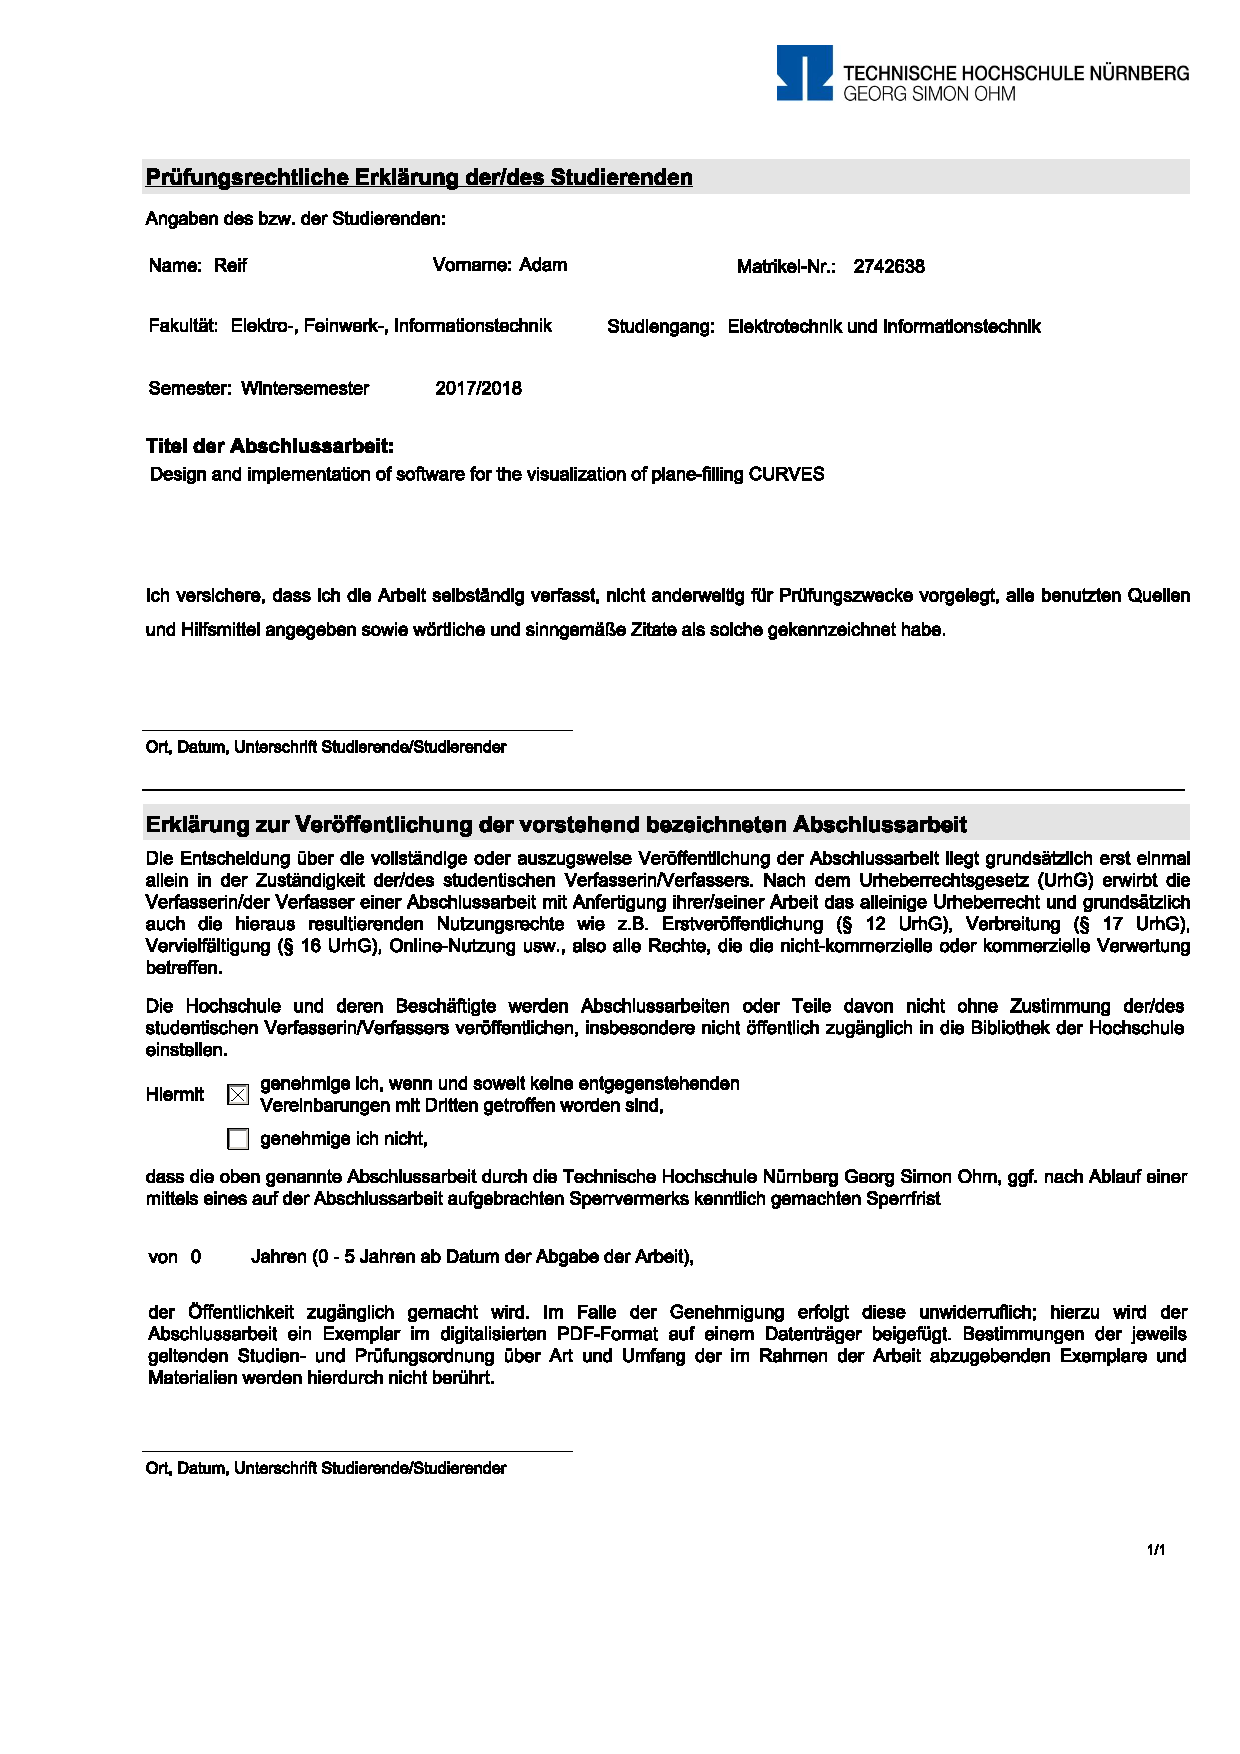
\includepdf[pages={1}]{erklaerung.pdf}

\ofoot{\pagemark}

% Seitennummerierung -----------------------------------------------------------
%   Vor dem Hauptteil werden die Seiten in großen römischen Ziffern 
%   nummeriert.
% ------------------------------------------------------------------------------
\pagenumbering{Roman}
%%\section*{Zusammenfassung}
%\label{sec:Zusammenfassung}
%Lorem ipsum dolor sit amet, consectetuer adipiscing elit. Quisque Natural"=Programmierung blandit sed, hendrerit at, pharetra eget, dui. Sed lacus. Pellentesque malesuada. Cras gravida mi id sapien. Ut risus justo, fermentum non, scelerisque sit amet, lacinia in, erat. Proin nec lorem. Quisque porta, nisl at porta aliquam, felis libero consequat ipsum, vitae scelerisque dolor mi a odio. Cum sociis natoque penatibus et magnis dis parturient montes, nascetur ridiculus mus. Duis sollicitudin. Proin sollicitudin varius arcu. Morbi eleifend, metus sit amet placerat pharetra, dolor dui lobortis pede, vel imperdiet tellus eros imperdiet lorem. In hac habitasse platea dictumst. Curabitur elit mi, facilisis nec, ultricies id, aliquet et, magna. Cum sociis natoque penatibus et magnis dis parturient montes, nascetur ridiculus mus. Aliquam ac est. Mauris turpis enim, feugiat non, imperdiet congue, scelerisque non, purus. Lorem ipsum dolor sit amet, consectetuer adipiscing elit. Nullam dictum aliquet purus. Maecenas faucibus. Maecenas suscipit.


\section*{Abstract}
\label{sec:Abstract}
%Fusce neque est, tincidunt eu, nonummy nec, tempor iaculis, erat. Lorem ipsum dolor sit amet, consectetuer adipiscing elit. Vestibulum egestas, velit a rhoncus gravida, metus dolor pulvinar diam, sit amet placerat risus dolor sit amet elit. Maecenas eget purus ut est mattis porta. Suspendisse ut mi et mauris lobortis malesuada. Vestibulum dapibus. Duis hendrerit, elit eu venenatis eleifend, sapien ante volutpat odio, ac condimentum tellus massa ut massa. Etiam dapibus imperdiet metus. Sed sapien arcu, pulvinar quis, laoreet quis, venenatis non, justo. Aliquam est ante, pulvinar nec, accumsan sed, auctor sed, augue.

%Ut adipiscing ligula. In mattis. Ut varius. In nec nulla at eros molestie viverra. Duis dolor risus, lobortis vel, dictum a, pellentesque id, lectus. Sed suscipit orci ac ligula venenatis condimentum. Maecenas et sem lacinia tortor cursus tempus. Mauris pellentesque risus at nulla. In arcu. Curabitur mattis mi quis dolor. In leo. Vivamus ut libero.
 - Guideline does not want an abstract, so they dont get one
\tableofcontents % Inhaltsverzeichnis

% Abkürzungsverzeichnis --------------------------------------------------------
\label{sec:Glossar}
% für korrekte Überschrift in der Kopfzeile

\listoffigures % Abbildungsverzeichnis
\listoftables % Tabellenverzeichnis
\lstlistoflistings % Listings-Verzeichnis
\printglossaries

% arabische Seitenzahlen im Hauptteil ------------------------------------------
\clearpage
\pagenumbering{arabic}

% die Inhaltskapitel werden in "Inhalt.tex" inkludiert -------------------------
% Hier können die einzelnen Kapitel inkludiert werden. Sie müssen in den 
% entsprechenden .TEX-Dateien vorliegen. Die Dateinamen können natürlich 
% angepasst werden.

\chapter{Introduction}
\label{cha:Intro}

\section{Field of Research}

Fractal geometry is an area of mathematical research that concerns itself with mathematically describing n-dimensional geometries - limited here to geometries on a plane - that display \textit{interesting} characteristics. 

Figure \ref{fig:flosnek} shows a rendering of one such geometry called \textsc{Gosper's flowsnake}.
It is a single, uninterrupted curve on a triangular grid, which is

\begin{description}
	\item [self similar] The macroscopic behaviour of the curve is the same as its microscopic behaviour
	\item [self avoiding] The curve is made from one continuous line that never intersects with itself.
	\item [edge covering] The curve travels across every cell of its grid, i.e. it fills up a given, arbitrary area completely
	\item [plane filling] The curve grows outward on the 2D plane without bounds. Infinitely iterated it covers the full plane.
\end{description}

\begin{figure}[h]
\centering
\begin{subfigure}{.33\textwidth}
  \centering
  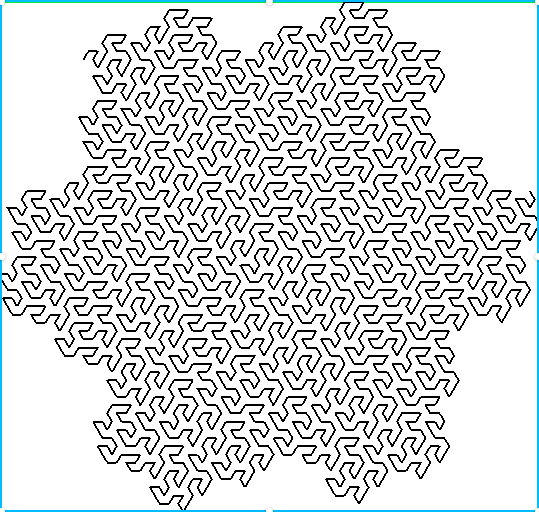
\includegraphics[width=.7\linewidth]{flosnek_4it}
  \caption{4 iterates}
\end{subfigure}%
\begin{subfigure}{.33\textwidth}
  \centering
  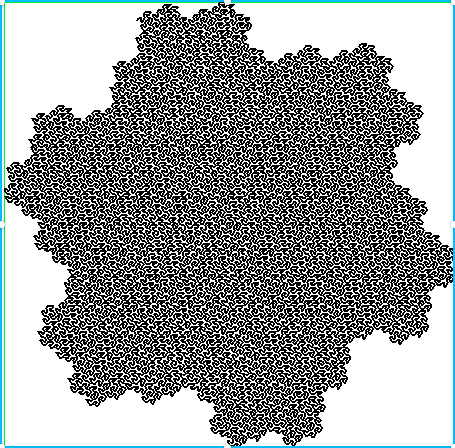
\includegraphics[width=.7\linewidth]{flosnek_5it}
  \caption{5 iterates, rescaled}
\end{subfigure}%
\begin{subfigure}{.33\textwidth}
  \centering
  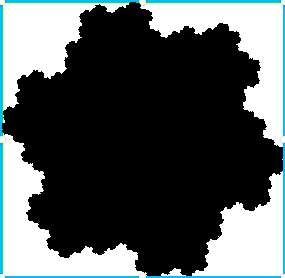
\includegraphics[width=.7\linewidth]{flosnek_8it}
  \caption{8 iterates, rescaled}
\end{subfigure}
\caption{Rendering of \textsc{Gosper's flowsnake}, with \gls{bounding box}}
	\label{fig:flosnek}
\end{figure}

The curve is obtained by iterating a so-called \gls{lsys}.

Originally introduced by biologist \textsc{Aristid Lindenmayer} in 1968 "as a foundation for an axiomatic theory of development" of plants \citep[Preface]{Prusinkiewicz2013}, it was found to be a useful language for describing a wide class of fractal geometries.
An \gls{lsys} consists of an inital string - the \textit{\gls{axiom}} - which is manipulated via a set of substitution \textit{rules}, the result of which is a called the first \textit{production} or \textit{iterate} of the \gls{lsys}. Subsequent iterations are generated by applying the \textit{rules} to the current \textit{production}.

The \gls{lsys} for figure \ref{fig:flosnek} is given in \citet[p.7]{Arndt2016} to be 
\begin{quote}
	\centering
	L $\rightarrow$ L+R++R-L- -LL-R+ \quad and \quad R $\rightarrow$ -L+RR++R+L- -L-R
\end{quote}
starting with an \textit{\gls{axiom}} of L. The first iterate of \textsc{Gosper's flowsnake} thus becomes L+R++R-L- -LL-R+, as the initial \gls{axiom} L gets substituted as per the left rule. 

The characters in this string are given special meaning w.r.t. to the curve:
\begin{description}
	\item[Alphabetic character] Denotes drawing a line from the current position forward by on a defined length. Forward being defined as the current direction
	\item[+ -] Characters denoting changes in direction by a set amount, e.g. in figure \ref{fig:flosnek} by $\pm60^\circ$, creating a triangular grid of movement
\end{description}

Those rules define a way to render a curve given by a \textit{\gls{product}}, and can be extended by other, auxilliary characters, discussed in \ref{sec:implementation}, e.g. \_ which changes color of subsequent segments.

\begin{figure}[hb]
	\centering
	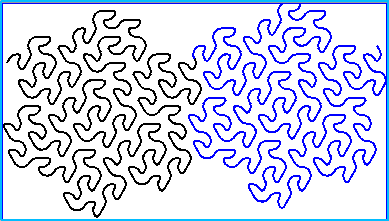
\includegraphics[width=0.5\textwidth]{flosnek_color}
	\caption{3-iterate rendering of \textsc{Gosper's flowsnake} with axiom \textrm{L\_L} and a rounding factor of 0.5}
\end{figure}

\section{Problem Statement}
In 2016, Prof. Jörg Arndt, the supervisor of this thesis, conducted research on finding plane-filling curves for \gls{lsys} with one non-constant character and published an article \citep{Arndt2016}, where he presented 2D renderings of the curves found.

The tools used to get from an \gls{lsys} description to a graphical, pdf-embeddable rendering of the iterated curve were assortments of chained commandline scripts, leaving much to be desired in flexibility and ease-of-use.

Thus, a request was issued for the creation of a \emph{cross-platform, maintainable and extensible} software that is able to create, visualize and export \gls{pfc}s from their \gls{lsys} descriptions.

\section{Approach}

Since this problem is multi-faceted, and the additional requirements introduce significant complexity on top of the "implement a renderer/exporter" core task, a structured approach to finding a solution is taken using decomposition methods from software engineering.

First, the requirements are formulated and discussed.

Then, research is conducted on available technologies for satisfying given requirements.

An architectural model is created using \gls{uml} to define the system architecture.

This model ist then implemented and refined/amended to address issues arising during the implementation process.

The software is tested during development with \gls{ci} and \gls{unit test} techniques.

Finally, a short investigation of application performance is conducted.

\section{Requirements to a Solution}
The following requirements to a satisfactory solution are given in figure \ref{fig:directreq} with a supposed workflow shown in the use-case diagram \ref{fig:uc}

\begin{figure}[h]
	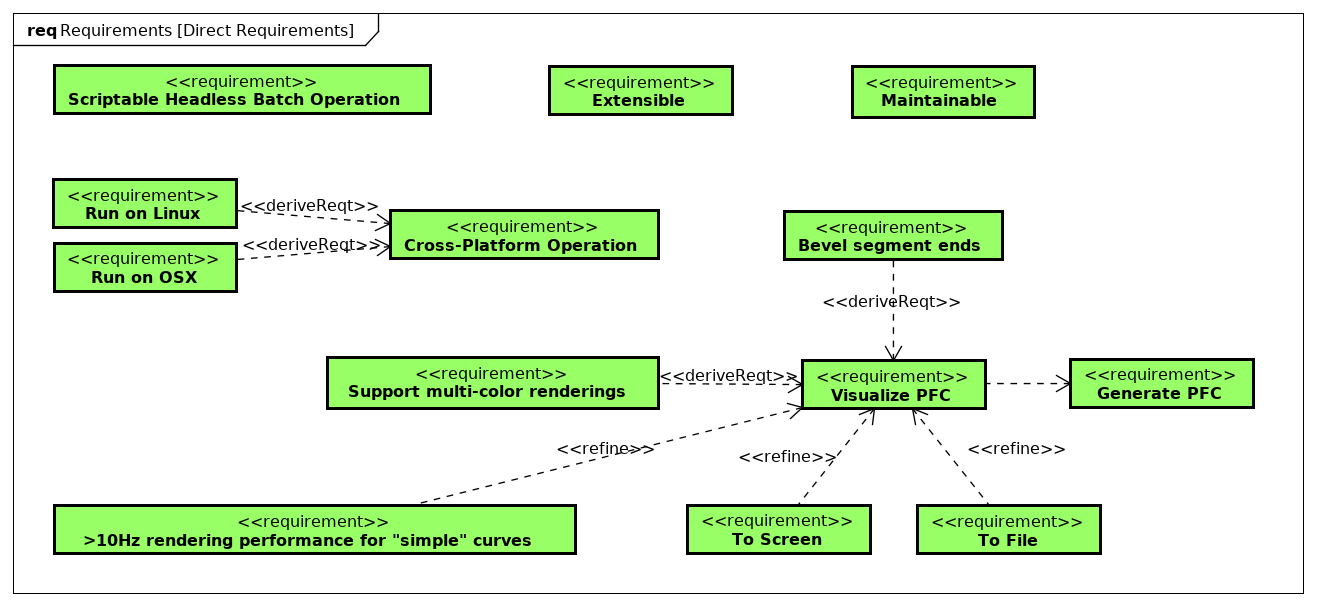
\includegraphics[width=\textwidth]{DirectRequirements}
	\caption{Direct user requirements to a solution}
	\label{fig:directreq}
\end{figure}


\begin{figure}
	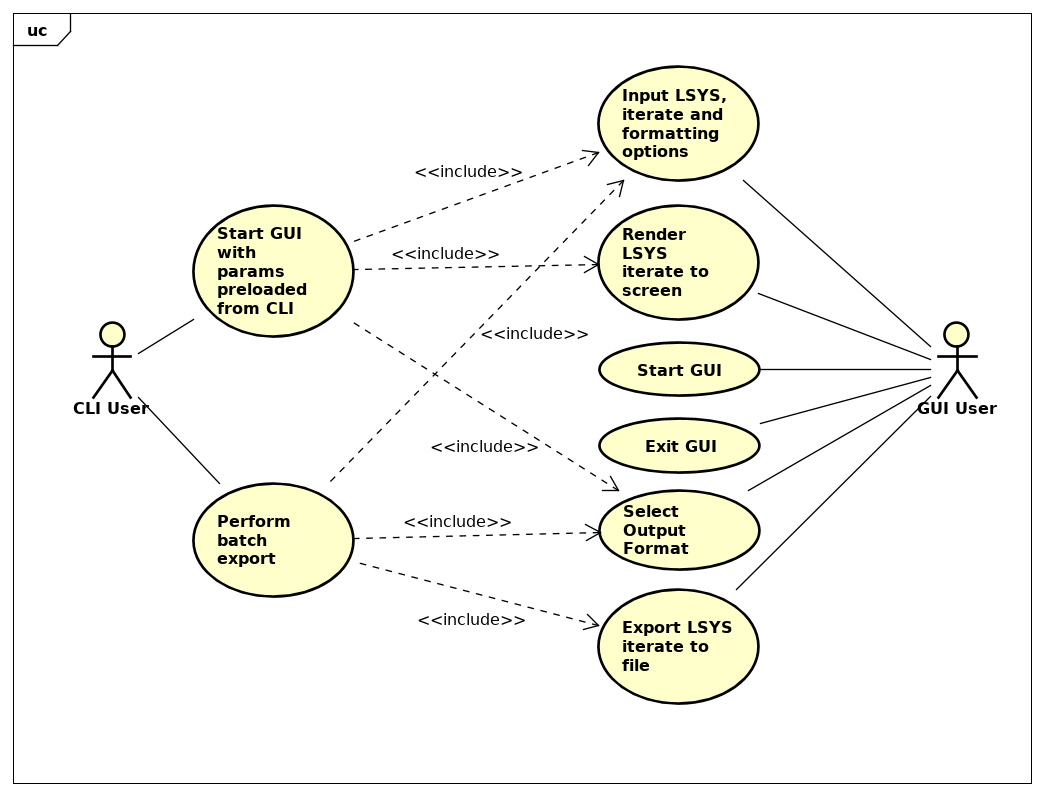
\includegraphics[width=\textwidth]{UseCaseDiagram}
	\caption{Workflow with the pfcrender tool}
	\label{fig:uc}
\end{figure}

These requirements are discussed in detail in the following sections and an architecture is formulated that satisfies them.

\chapter{Research and Architecture Definition}

\section{State-of-the Art Development Environment}

Maintainability was declared a main goal in the requirements, and this is an issue with much broader reach than just good programming practice.

It consists of many non-coding factors such as

- ease of collaboration, issue tracking
- enforcing of good coding by-default, e.g. through static analysis
- early indication of breaking changes
- incremental integration or big-bang-release
- ease of code documentation

The importance of such "meta-programming" techniques is testified by the fact, that a job field for software engineers called \gls{DevOps} exists, which engages in finding ways to optimize coding workflow all day.

\subsection{Version Control}

\subsubsection{Git}
\gls{git} is an code revisioning software implementation created by Linus Torvalds, searching for a solution to manage the growing base of coders on his main project - the \gls{linux} kernel.

Its key benefits are
- Decentralization: No reliance on a central server for daily work
- Smart Merging: Conflict resolution algorithms are fairly good at finding and automatically fixing trivial conflicts, keeping developer interaction a merge to a minimum
- Central repository supported: Though git operates locally, it supports pushing code to and pulling from remote repositories, enabling the use of a central "synchronization" repository, which is the Basis for the popular \gls{github} 

\subsubsection{SVN}
A revisioning software once claiming to be "CVS done right", where CVS is its direct precursor.

It is a  
\subsubsection{Mercurial}

\subsection{CI}
Continuous Integration is a concept popularized as an \gls{agile} method
\subsubsection{Github}

\subsubsection{Jenkins}


\subsection{Unit Testing frameworks}

"nobody has the time to write tests"

\subsection{Model-driven Design and Round-Trip Engineering}
Modeling is often the first step of implementing a fairly complex architecture, 

decomposing the goal into subobjectives and defining clear interfaces, enabling parallel execution when working in a team.

UML

Models - when, like documentation, manually created - are cumbersome to maintain and keep synchronized with necessary changes to the architecture discovered during implementation.

In classic Model-driven Design, the UML model can be used to generate boilerplate parts of the code (e.g. class / namespace declarations) to save the implementers some work.

Architectural changes made in the code have to be manually introduced in the model as well, which can not be enforced and often leads to the model desyncing. Because of that, often a waterfall model of project design is adopted, where the model is created as a starting point of implementation, and after it has been reviewed and implementation begins, discarded.

Round-Trip Engineering Tooling helps alleviate this problem, by automatically feeding changes from the code back into the UML model.

Depending on the target language, the task of reintroducing changes can be very difficult. C++, being a very syntactically complex language is notoriously difficult to round-trip engineer, reflecting in bad tool support.o

%TODO: list of tools that claim to offer c++ rountripping

- Astah - plugin


Since no suitably sophisticated tool could be identified in the noncommercial solutions, round-trip engineering could not be used in this project.


\subsection{Autogenerated Docs}


\section{Software Architecture Considerations}

\subsection{Plugin Architecture}
Looking at the requirements, it is apparent, almost all component have disjunt responsibilities, their main common element being the string description of the PFC they operate on.

The \gls{lsys} generator takes some input and outputs a model string. GUI, SVG and PDF renderings all operate on the model, but don't influence each others operation.

This characteristic is conducive to segregating those components of the app not just to different classes, but to completely separate compilation units, i.e. standalone libraries called plugins.

In conjunction with a dynamic loading system, this confers several benefits:

- Reduced compilation time of the main application
- Extensibility without recompilation
- 

This architecture also comes with drawbacks
- Updating the main app with changes breaking public APIs used by plugins will fail at runtime until all plugins have been updated/recompiled
- If plugins have dependencies on other plugins, maintenance complexity grows exponentially and loading sequence must be enforced

The additionally introduced complexity can - in sufficiently complex projects - significantly outweigh modularization benefits, resulting in what is called \"plugin hell\". %\ref @ph.
The Eclipse IDE, in its core being a plugin loader and all functionality supplied by plugins is a prime example of the possible complexity.

Since plugins to pfcrender will mainly consist of new Import/Export formats with limited intrinsic complexity and no dependencies on other plugins, a plugin architecture was deemed beneficial for increasing extensibility and thus the following architecture was chosen.

%\image {Plugin architecture}

\subsection{Configuration}
Main considerations:
- Want all options to be command line selectable
- Want documentation of available commandline options
- Options are provided by components of the GUI as well as by plugins

The main interface to the application will be the commandline.

Automatic documentation of all available options to the commandline is a must-have feature when maintainability of the application is a major concern.

Though other, manual approaches like manfiles and README documents exist, it is not only difficult to prevent them from desynchronizing with the actual code of the program, in a plugin architecture as described above, the actual functionality offered by the total of available plugins will vary by deployment and can thus not be centrally written down.

It was thus decided to introduce a central store of configuration, that will be accessible to the entire application.

Furthermore, each plugin is required to publish configuration options it needs to the main application.

Since all available commandline options must be known at parsing time for documentation generation and parsing itself, it follows that all plugins must be loaded once on startup to query them for their config options.

While this is not computationally efficient, as not all plugins will necessarily be executed during program runtime and thus get loaded in vain, maintainability outweighs this minor performance issue, as the number of plugins is small

%TODO: Make callgrind timing analysis of lib calls 

A standard workaround for this issue is builing a list of options at compile time, e.g. using the C++11 constexpr keyword or \gls{tmp}, this method is not suitable here, since options available depend on the available plugins, which are only known at runtime.
See also \url{https://stackoverflow.com/questions/9975672/c-automatic-factory-registration-of-derived-types}
or auto registration of class with a typelist ?
\url{https://stackoverflow.com/questions/42077057/c14-metaprogramming-automagically-build-a-list-of-types-at-compile-init-tim?rq=1}

Another problem is gathering options from plugins automatically is possible when building a list of plugins, options exposed by the main application can not be added this easily, as the objects that expose the info structure do not need to exist by the time. So in this instance - for options of the main app - a manual list must be maintained after all. While this difference in behaviour betwenn core and plugins is unfortunate, it is still an improvement over fully manual API documentation.

For further details on the implementation, see \ref chapterX{Singleton}

This central store can also be exposed to user via the GUI (see \ref chapterX{guiconfig}

\subsection{Batch mode}
Unlike in the GUI, where we can check for config options once the object using them is instantiated, the CLI batch mode runs a preset sequence of steps and needs to gather all available/acceptable config options before starting the process in order to generate meaningful CLI documentation.	

\subsection{config stores}
The selected architecture defines an order of precedence of config options:
1. Global options are set from config file is parsed
2. options given on Command line are set 
(3. GUI options can set config settings)

\subsection{Performance}
\subsubsection{fxtlib}
\subsubsection{move semantics when operating on model}

\subsection{Cross-Platform Operation}
\subsubsection{Qt Framework}
QApplication, main event loop

\subsubsection{Dynamic Library Loading}
POSIX Systems use dlopen()

Windows uses LoadLibrary()

To get cross-platform operation without recompiling, use Qt's Library loading mechanism: QPluginLoader

\subsubsection{QtQuick}
QML integrate in C++

QRC QtResourceCollection

qml files are not compiled (javascript like)
Actually based on ECMAScript6 aka. JavaScript

declarative as opposed to the imperative  C++

\subsubsection{Signals and Slots in QML}
Signals are captured by invoking Signal Handlers

\subsubsection{Qt and C++1y}
Move semantics not implemented
QQuickItem has disabled copy ctor and no move ctor
use unique\_ptrs to copy without resource leaks


\subsection{Extensibility}
\subsubsection{Plugin Structure}
Lower app startup times, not every importer exporter is needed on every app run

Easy to extend the app with new importers / exporters without touching other internal code

Plugins encapsulated by Shared Libraries can be published to the app, registry of available plugins can be read from config file.

No recompilation needed on adding/removing plugins.

Each plugin must share a common interface though

\section{Design Patterns}
\subsection{Registry Pattern}

\subsection{Factory Pattern}

\subsection{Builder Pattern}

\subsection{Singleton}
Single instance + easy global access from all classes of the app


\section{Problems}
\subsection{Model Creation}
QQuickPaintedItem uses a given painter, explicitly calling functions on it to draw on a paint device.
We want the finished image though, not something that draws based on input. We would need to embed the LSYS string into the model if that were the case.

Und jetzt habe ich die Wahl was ich in der GUI als Modell der PFC speichere, bisherige Überlegungen:
- Den String selbst
Die Ideen sind wohl halbwegs speicheroptimal, müssen aber wohl entweder ein ViewModel zwischengeschaltet bekommen, bevor sie renderbar werden, was den Speichervorteil zunichte macht, oder auf ein Canvasobjekt "gemalt" werden
- Als SVG. Einfach zu rendern, aber den SVG overhead zu parsen ist sicher alles andere als performant.

Model: - 2D - Matrix in der jeder Index ein Segment mit Richtung und Farbe repräsentiert

- Ein QML-Objekt (QQuickPaintedItem), das den LSYS String als member enthält und neu zeichnen lässt (bessere Austauschbarkeit des Modells - nicht limitiert auf PFCs)
- Ein generisches QQuickItem, das als Information direkte OpenGL drawing calls enthält (QSGGeometry)

Das Model muss weiterhin nicht nur als Bitmap renderbar, sondern in verlustfreier Form z.B. nach SVG exportierbar sein - die Daten z.B. nur in einer QSGGeometry vorzuhalten ist praktisch zum rendern (automatisch in Qt), aber unmöglich aus dem Quickitem wieder zu extrahieren


\section{Chosen Application Architecture}

%\figure{fullrequirements.png}



\section{Flexible Buildsystem}
Due to the requirement of a Multi-platform architecture, one of the first considerations is how to get the program code built.

Though it would surely be possible to have the platform agnosstic sources present, and then manually create a project for MSVC/MinGW when on Windows, gnu gcc on Linux and clang on Mac, this would be a pain to set up and maintain.

Solutions to this problem exist in so-called buildsystem generators. Those gather sources, dependencies and additional project information from a configuration file, detect the architecture they are running on, and generate the files necessary to compile the full project on whichever compiler is present on the current system.

QMake - The native buildsystem generator of Qt, uses .pro files for project description

CMake - A powerful and scalable config script-driven generator that is widely used in both Open Source and commercial projects 


\section{Commandline Parsing}
Unlike other programming languages (e.g. Python), C++ does not provide a standard built-in facility to provide parsing capability for parsing parameters passed to the program as commandline options.

Alternatives:

\begin{itemize}
\item getopt() - Coming from C, this is a legacy method widely used on Linux. Since it is specific to POSIX systems, it cannot be used on Windows 
\item Boost.progam\_options - A C++ native, highly configurable solution shipped with the open source Boost library
\url{http://www.boost.org/doc/libs/1\_58\_0/doc/html/program\_options.html}
\item QtCommandLineParser - A Qt native parsing class. Batch-parses all parameters and returns data structures with positional arguments in correct order, and a (reordered) map of switches with their parameters
http://doc.qt.io/qt-5/qcommandlineparser.html
\item Manual parsing of the argv array. While this is the most flexible solution in customization, it is reinventing the wheel and also very inflexible with respect to extensibility.
\end{itemize}

Due to it supporting our use-case, being easily extensible and not introducing any more dependencies into the project above the already used Qt Framework libraries, the QtCommandLineParser was chosen to provide the main CLI-based interface to the program.


\section{Option Persistency}
Since it is often unneccessary to set any and all config options for the program on the command line each time it is run, keeping config options persistently over program relaunches is useful. The typical implementation of this persistent store again varies by platform, ranging from putting keys into the Windows registry, over property list files on Mac to plain .ini or .cfg files on Linux.

Again, Qt comes with a wrapper around this platform disparity

\chapter{Chosen Application Architecture}
After researching available technologies, an architecture to build the pfcrender tool on is selected from the alternatives found. It is shown alongside the original requirements in the following graphs, split between functional- (figure \ref{fr}) and non-functional (figure \ref{nfr}) requirements. As in figure \ref{fig:directreq}, direct requirements are highlighted in green. Note that each direct requirement is satisfied or verified through an implementation requirement or test case.

The architecture is discussed in detail in the following sections.

\begin{figure}[p]
	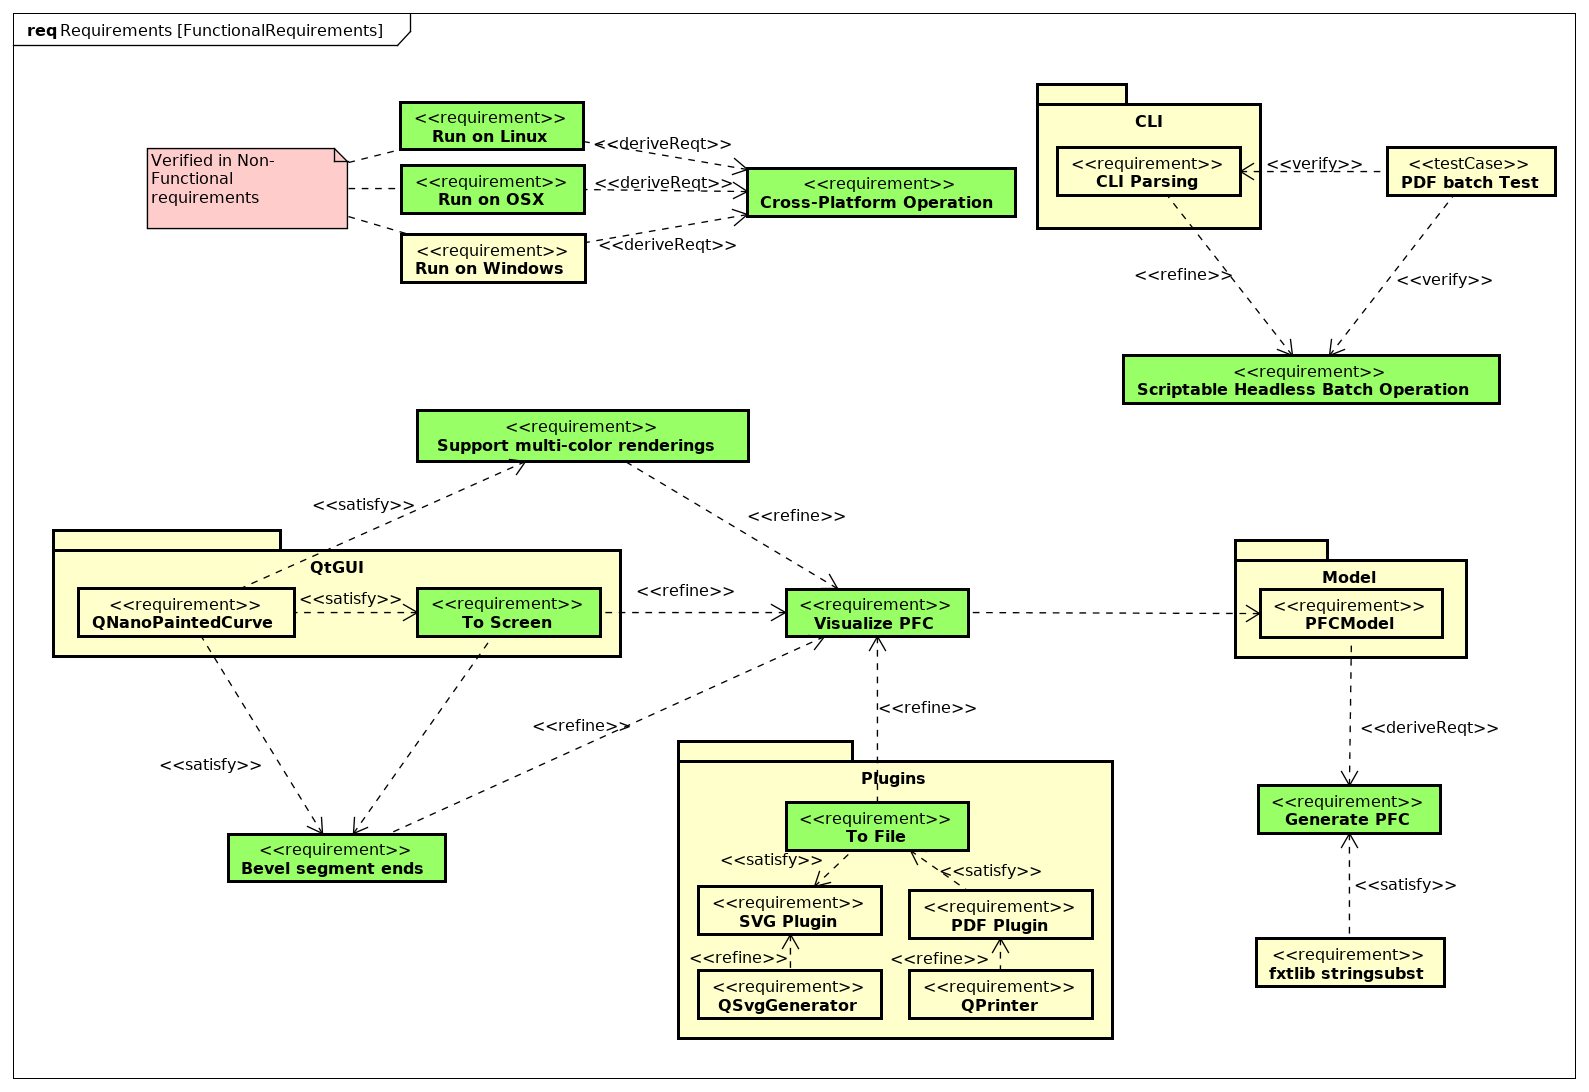
\includegraphics[width=\textwidth]{FunctionalRequirements}
	\caption{Functional requirements}
	\label{fr}
\end{figure}

\begin{figure}[p]
	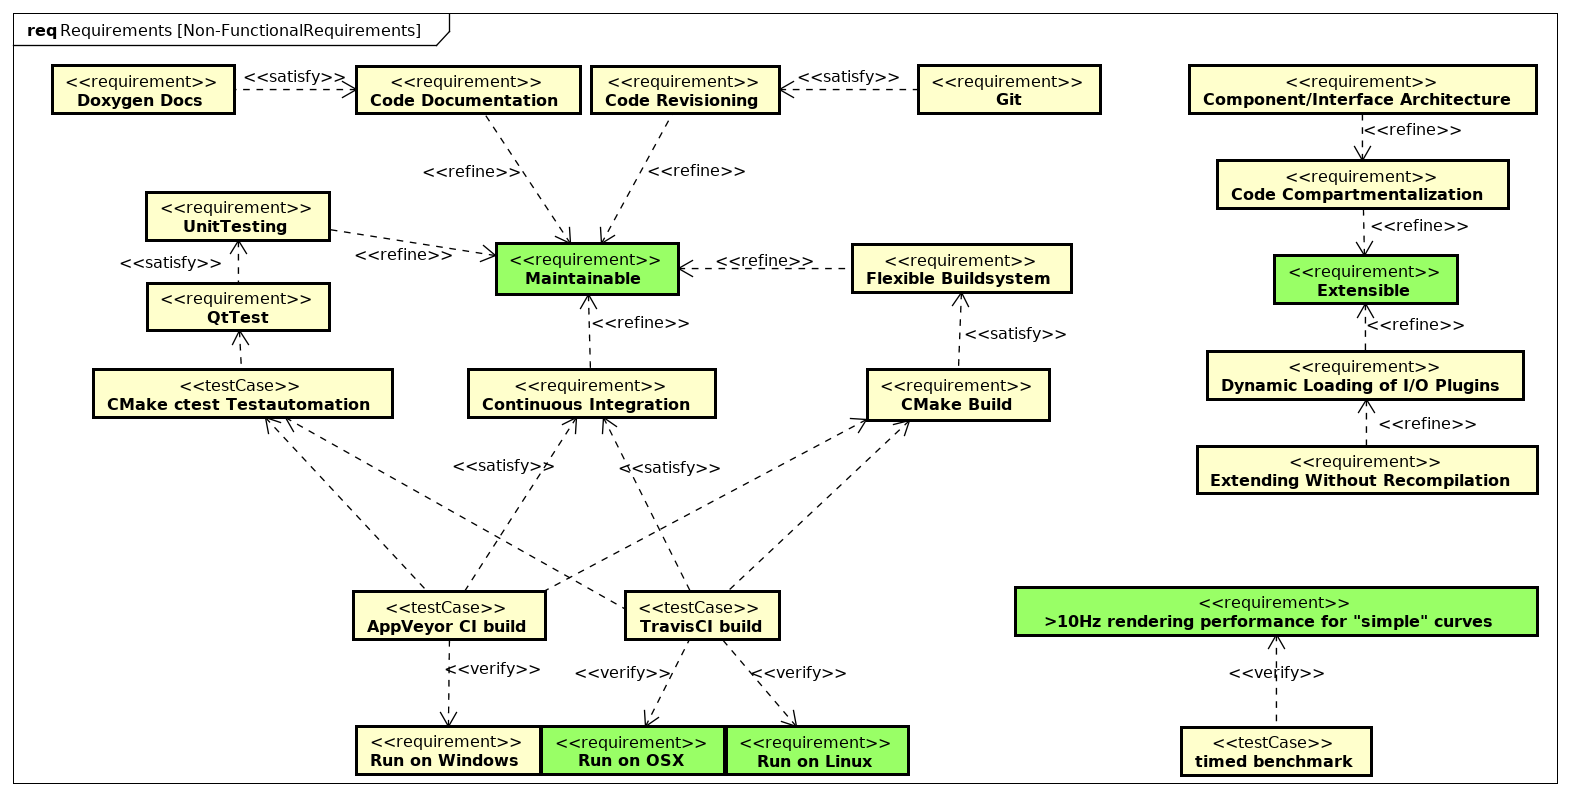
\includegraphics[width=\textwidth]{Non-FunctionalRequirements}
	\caption{Non-functional requirements}
	\label{nfr}
\end{figure}

\section{Functional Requirements}
The decision with the widest implications to the software architecture is selection of the appropriate graphics framework library from the ones discussed in section \ref{sec:res_frameworks}.
Selection was driven by three main concerns: \emph{extensibility, performance and ease-of-use}.

Ultimately, the Qt Framework was chosen for the following reasons:
\begin{itemize}
	\item Platform-independent dynamic library loading abstraction provided, which is useful for implementing a plugin architecture as described in section \ref{sec:resplug}
	\item Classes provided for exporting e.g. to SVG and PDF
	\item The QtQuick API exposes direct OpenGL access, i.e. rendering performance is assumed to be comparable to the more light-weight frameworks like \gls{sdl}
	\item Multiple quality-of-life improvements like the QtCreator \gls{ide} with \gls{gui} designer
	\item Included QtTest Unit-Testing Framework
\end{itemize}

Qt provides most of the wanted features in one framework, reducing the amount of necessary dependencies to provide all required functionality. The only additional dependency to Qt introduced to the project is the drawing \gls{api} QNanoPainter(\ref{sec:qnanopainter}), which was introduced as manipulating OpenGL geometry directly proved unwiedly for rendering arcs (see \ref{sec:implrenderprob})

A description of the Qt provided mechanisms used in this tool follows.

\subsection{Dynamic Library Loading}
Windows DLL API mandates symbols callable from outside a library to be prefixed with a macro on export and import. The \gls{msdn}\furl{https://msdn.microsoft.com/en-us/library/3y1sfaz2.aspx} defines it the following way
\begin{lstlisting}
__declspec( dllimport ) declarator  
__declspec( dllexport ) declarator  
\end{lstlisting}

Linux compilers like gcc will not be able to parse this keyword and fail compilation. While it is possible to work around this issue by wrapping the keyword in a preprocessor macro that expands to nothing on Linux, this mechanism is cumbersome to implement.

Qt provides a wrapper around this functionality with a class called QPluginLoader\furl{http://doc.qt.io/qt-5/qpluginloader.html}.

Making a library compatible to use with this mechanism involves some extra steps compared to loading a shared library directly, which pertain to making the Qt \gls{mos} aware of the plugin\furl{http://doc.qt.io/qt-5/plugins-howto.html}, but spares the effort of including platform specific adapter code/preprocessor instructions to each plugin.

\subsection{Rendering in Qt}
\label{sec:qtrender}
As stated before, Qt offers two different application programming \gls{api}s. A main difference is in the rendering methode they use:
\begin{description}
	\item [QWidgets] The main API of Qt. It is similar to Java SWING and handles \gls{gui} design and functionality in C++ using Qt-provided or custom QWidget-derived classes. Each widget handles rendering itself.
	\item [QtQuick] A relatively new (since Qt 4.7) javascript-based declarative language called \gls{qml}, similar to the XML-based JavaFX, is used to define the \gls{gui} frontend, while C++ classes in the backend are used for performance intensive calculation. Drawing information of QQuickItems is composed to a scenegraph, which is then handed to the platform specific graphics backend like OpenGL or OpenGL ES for rendering. Though no formal study of performance differences between both \gls{api}s exists, documentation by the QtCompany\furl{http://doc.qt.io/qt-5/qtquick-performance.html} suggests performance between both models is comparable if some guidelines are followed.
\end{description}

Since the additional model-/view abstraction is conducive to extensibility of the tool, as the declarative \gls{qml} language makes \gls{gui} extensions simple, QtQuick is selected for the implementation.

The following methods of drawing to these APIs are offered:
\begin{description}
	\item [QPainter] Oldest drawing API of Qt used in QWidgets. Offers a high-level API (e.g. drawLine(), drawArc() ), is not directly usable in QtQuick though. Offers highest amount of integration to other Qt classes (notably QPrinter and QSVGGenerator)
	\item [QtQuick/QML shape] Placing line segments directly in a \gls{qml} file and loading it to the SceneGraph (creating quadratic bezier curves added in Qt 5.10 (late 2017), too late to consider for this work\furl{https://blog.qt.io/blog/2017/08/10/let-there-be-more-shapes/})
	\item [QtQuick HTML5 canvas] Draws on top of a HTML5 canvas embedded into the qt app.
	\item [QtQuickItem with custom scene graph node] Instantiates a QQuickItem with custom appearance by directly setting vertices and material for the underlying OpenGL to render.
	\item [QQuickPaintedItem] An adaptation of the QPainter API for the SceneGraph based QtQuick. 
	\item [QNanoPainter]\furl{https://github.com/QUItCoding/qnanopainter} A third party plugin, offering a mixture of QPainter and HTML5 canvas API to draw on an OpenGL framebuffer object or QSGRenderNode to be placed in the QtQuick scene graph. Offers Painter-like productivity with less performance overhead.
\end{description}

The QML and HTML5 APIs were disregarded due to their interpreted and thus slow nature.

This leaves direct QuickItem implementation, QQuickPaintedItem and QNanoPainter-based QuickItem as viable options.

Due to performance measurements\furl{https://www.vikingsoftware.com/qtquick-custom-item-performance/}, a direct implementation was chosen intially (see \ref{sec:implQQuickItem}). The operations performed using this \gls{api} were too inflexible to allow for generation of quadratic bézier curves necessary to implement rounded edges, so a higher level \gls{api} was selected.

Further performance benchmarks\furl{http://kgronholm.blogspot.com/2017/12/qt-510-rendering-benchmarks.html} led to preferring QNanoPainter over the built-in QQuickPaintedItem, even though it meant introducing an additional dependency into the project.

It is worth noting, that QPainter \gls{api} was still used for file outputs (see \ref{svg}, \ref{pdf}), where performance is not as critical, due to its integration with other Qt exporter classes.

\subsection{Configuration}\label{sec:archconf}
It was decided to introduce a central store of configuration that will be accessible to the entire application using the Singleton pattern discussed in section \ref{sec:ston}.

Each plugin is required to publish and read its configuration options from this central store.

We define the following possibilities of setting options to the central store, in order of execution and inverse order of precedence:
\begin{enumerate}
	\item Options and state information are read from disk
	\item Options can be given on the command line
	\item Options can be set from within the \gls{gui}
\end{enumerate}

\subsubsection{Persistent Filesystem Storage - QSettings}
The Qt framework comes with a provider for storing settings called QSettings. It abstracts the programmer from platform specific storage solutions of a configuration store and provides a simple \cmd{save()} and \cmd{restore()} \gls{api} for the backing store it manages on its own. Configuration data is made available as a map of configuration identifier and configuration value.

\subsubsection{Commandline Parsing - QCommandlineParser}
Parsing of the commandline is one of the first steps in program execution. Since successfully parsing given arguments (and generating documentation on available options accessible by running \cmd{pfcrender --help}) requires all available options to be known, it follows that all plugins must be loaded on startup to query them for their config options.

While this is not computationally efficient, as not all plugins will necessarily be executed during program runtime and thus get loaded in vain, maintainability outweighs this performance issue.
Loading all plugins is a once-per-execution process only delaying application startup, not normal operation. Also, the number of plugins is fairly small. A benefit of loading all plugins at startup allows for automatically gathering available functionality on startup, omitting the need for a separate configuration file of plugins and their locations.

It is thus defined that plugin libraries will be located in a Plugins subfolder below the binary executable that contains no files other than plugins, so they can be crawled and loaded each time the program executes.

This design allows for a \emph{self-documenting, truly runtime extensible} plugin system, where plugins can be added/removed from the program without additional configuration steps.

Due to it supporting our use-case, being easily extensible and not introducing any more dependencies into the project above the already used Qt Framework libraries, the QtCommandLineParser is chosen to provide the main CLI-based interface to the program.

A drawback of QCommandlineParser is batch parsing of the commandline, making it impossible to group configuration switches (denoted by - -switch syntax) by their position of occurrence in the argument string.

We thus define the following:
\begin{enumerate}
	\item Actions taken by the program shall be specified on the commandline as positional arguments (with no preceding \cmd{-}), to guarantee their execution in order
	\item configuration options are specified with - -prefix and shall be unique throughout the application (including all plugins)
\end{enumerate}

\subsubsection{GUI configuration - QQuickItem}
In order to make configuration possible from the \gls{gui}, a plugin shall expose a configuration screen described in \gls{qml} as a QQuickItem through its plugin interface, that contains all logic for setting configuration options on the plugin for the \gls{gui} to display.

\section{Non-functional Requirements}

\subsection{Qt Unit Testing Framework}
Qt comes with its own unit-testing framework integrated into QtCreator. The following code presents an example test for a fictional Counter class:

\begin{lstlisting}[caption=Unit Test for a Counter class,language=c++]
#include <QtTest>
#include "Counter.h"

class MyTest : public QObject {
    Q_OBJECT

    Counter* ctr;

private slots:
    void initTestCase();

    void do_count();
  //void do_downcount(); // additional test routines

    void cleanupTestCase();
};

void MyTest::initTestCase()
{
	ctr = new Counter(0);
}

void MyTest::cleanupTestCase()
{
    delete ctr;
}

void MyTest::do_count()
{
	ctr->count();
	QVERIFY(ctr->getValue() == 1);
}

QTEST_MAIN(MyTest)
#include "MyTest.moc"
\end{lstlisting}

This builds an executable (main routine provided by the QTEST\_MAIN macro) that runs the given test routines.
It is integrated with QtCreator, which gathers test executables created in this way automatically, can run them from the \gls{gui} and display PASS/FAIL status depending on QVERIFY() and return value as shown in figure \ref{fig:qtctest}.

Since it is a standalone executable, it can also be run by other testing environments like CMake's CTest, and thus be automated and integrated into \gls{ci} builds as shown in figure \ref{fig:travistest}
\begin{figure}[htb]
	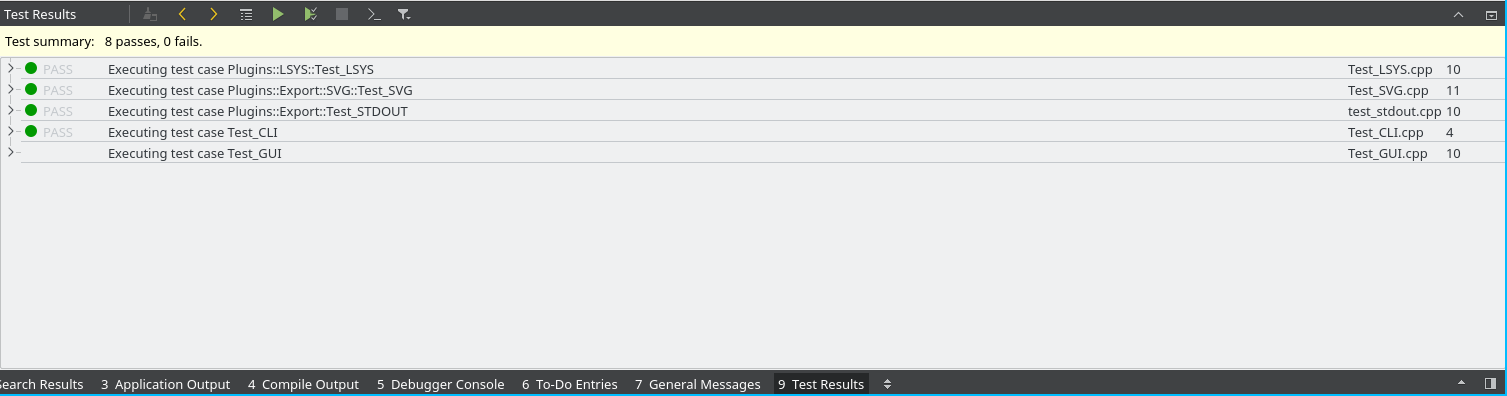
\includegraphics[width=\textwidth]{qtcreator_testing}
	\caption{Unit Testing Output of QtCreator}
	\label{fig:qtctest}
\end{figure}

\begin{figure}[htb]
	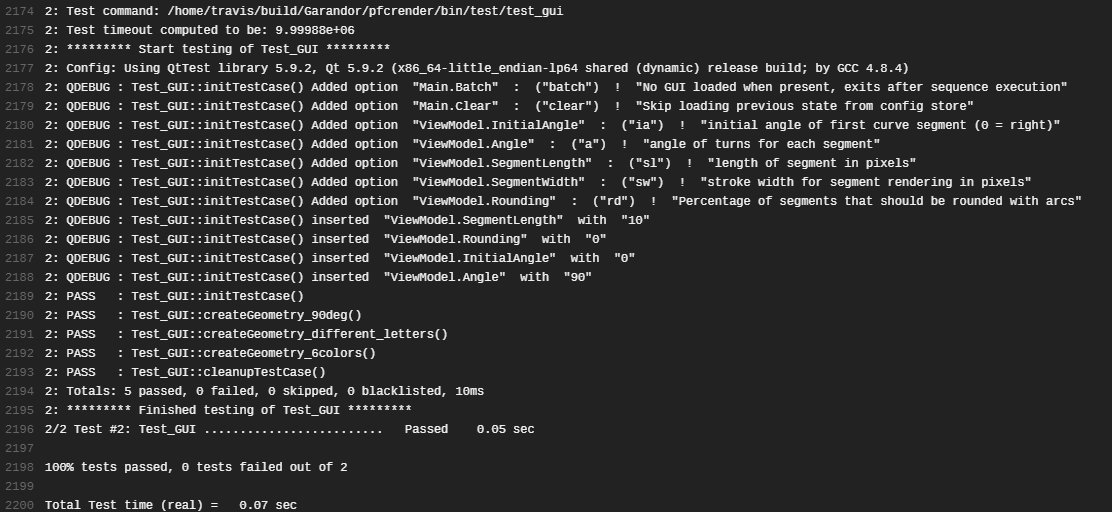
\includegraphics[width=\textwidth]{travis_testlog}
	\caption{Unit Testing Output of a \gls{ci} build using Travis CI}
	\label{fig:travistest}
\end{figure}

\subsection{Makefile Generator - CMake}
Though as described in section \ref{sec:resMakefileGen} Qt has its own makefile generator with qmake, CMake was selected for the following reasons
\begin{description}
	\item[Widespread Use] Though more feature-rich than QMake, CMake is extensively documented
	\item[CTest Test-Runner] Allows to define available unit tests in CMake configuration files and automatically run them after build completion 
\end{description}

Especially the test runner is a large gain for maintainability when integrated with \gls{ci} as shown in figure \ref{fig:travistest}, as it makes automated builds more informative.
A build will not only report failure on changes that break compilation, but also on changes that break runtime functionality for which tests exist. This in turn encourages contributors to actually write unit tests, since they don't need to be run manually.

\subsection{Version Control System}\label{sec:archvcs}
Due to the useful issue tracking feature of \gls{github} and its extensive third party infrastructure integration with services like \gls{ci}, \gls{git} is selected as \gls{vcs} and \gls{github} as the central repository provider.

The project can be found at \url{https://github.com/Garandor/pfcrender}

\begin{figure}[htb]
	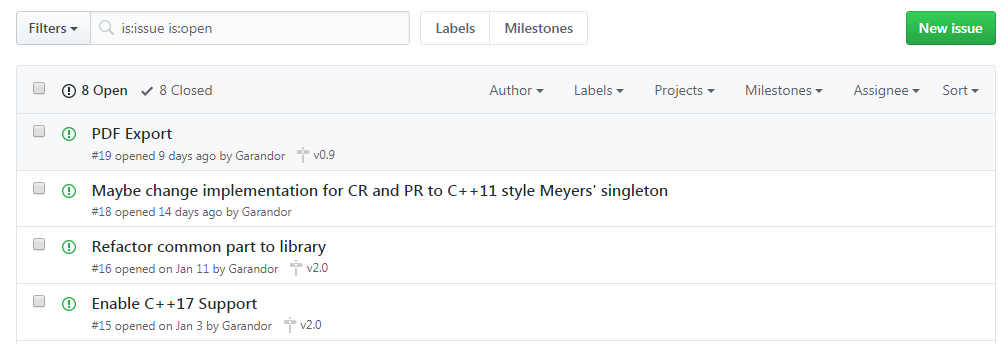
\includegraphics[width=\textwidth]{github_issues}
	\caption{GitHub issue tracking board}
	\label{fig:githubissues}
\end{figure}

We leverage \gls{github}'s integration by connecting it to the \gls{ci} providers Appveyor for windows builds, and Travis CI for Linux and MacOS X, due to their free-for-open source service.

\gls{ci} services for our repository are located at
\begin{itemize}
	\item \url{https://travis-ci.org/Garandor/pfcrender}
	\item \url{https://ci.appveyor.com/project/Garandor/pfcrender}
\end{itemize}

Furthermore, \gls{ci} runs are used to run a CTest suite of unit tests generating \gls{coverage} reports as described in section \ref{sec:autotest}, which are then uploaded to cloud coverage dashboard codecov.io at \url{https://codecov.io/gh/Garandor/pfcrender}.

\begin{figure}
	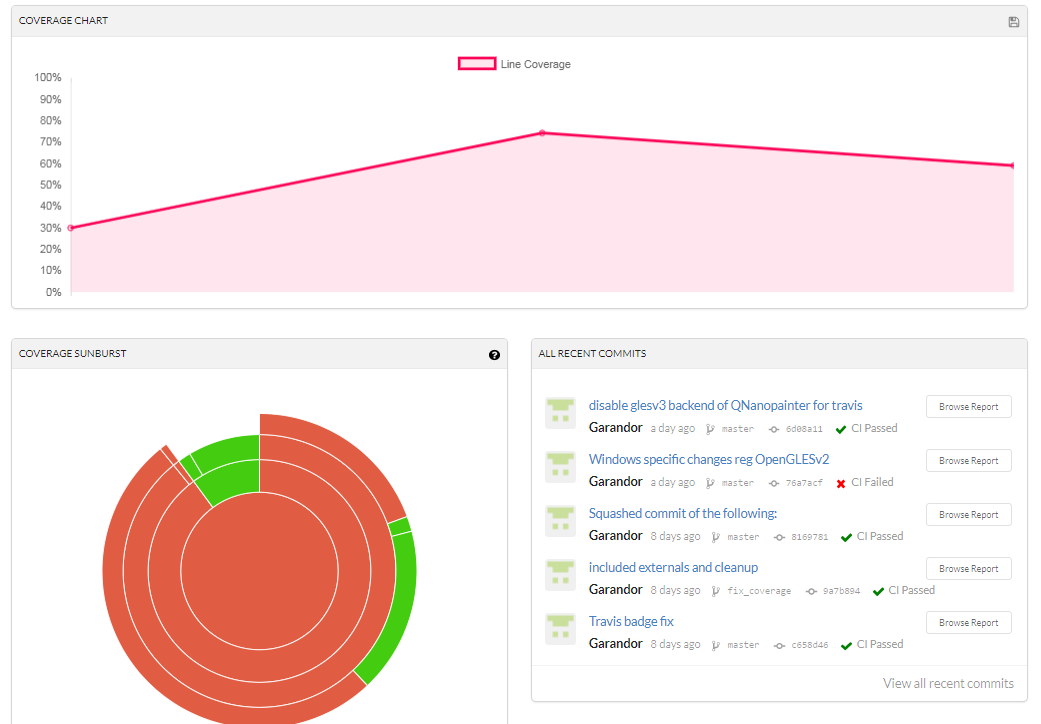
\includegraphics[width=\textwidth]{codecov.png}
	\caption{Codecov.io coverage dashboard}
	\label{fig:codecov}
\end{figure}

Documentation for this project is automatically generated from Doxygen structured comments in the code (see sec. \ref{sec:resdoxygen}) on every \gls{ci} build of the master branch on \gls{github}, which is then uploaded to github-pages, a website/documentation hosting service of \gls{github}\furl{https://pages.github.com/}.

It is located at \url{https://garandor.github.io/pfcrender/}

All of the additional services are linked from the repository's mainpage for easy access.

\section{Architecture Hierarchy}\label{sec:archplug}
\begin{figure}
	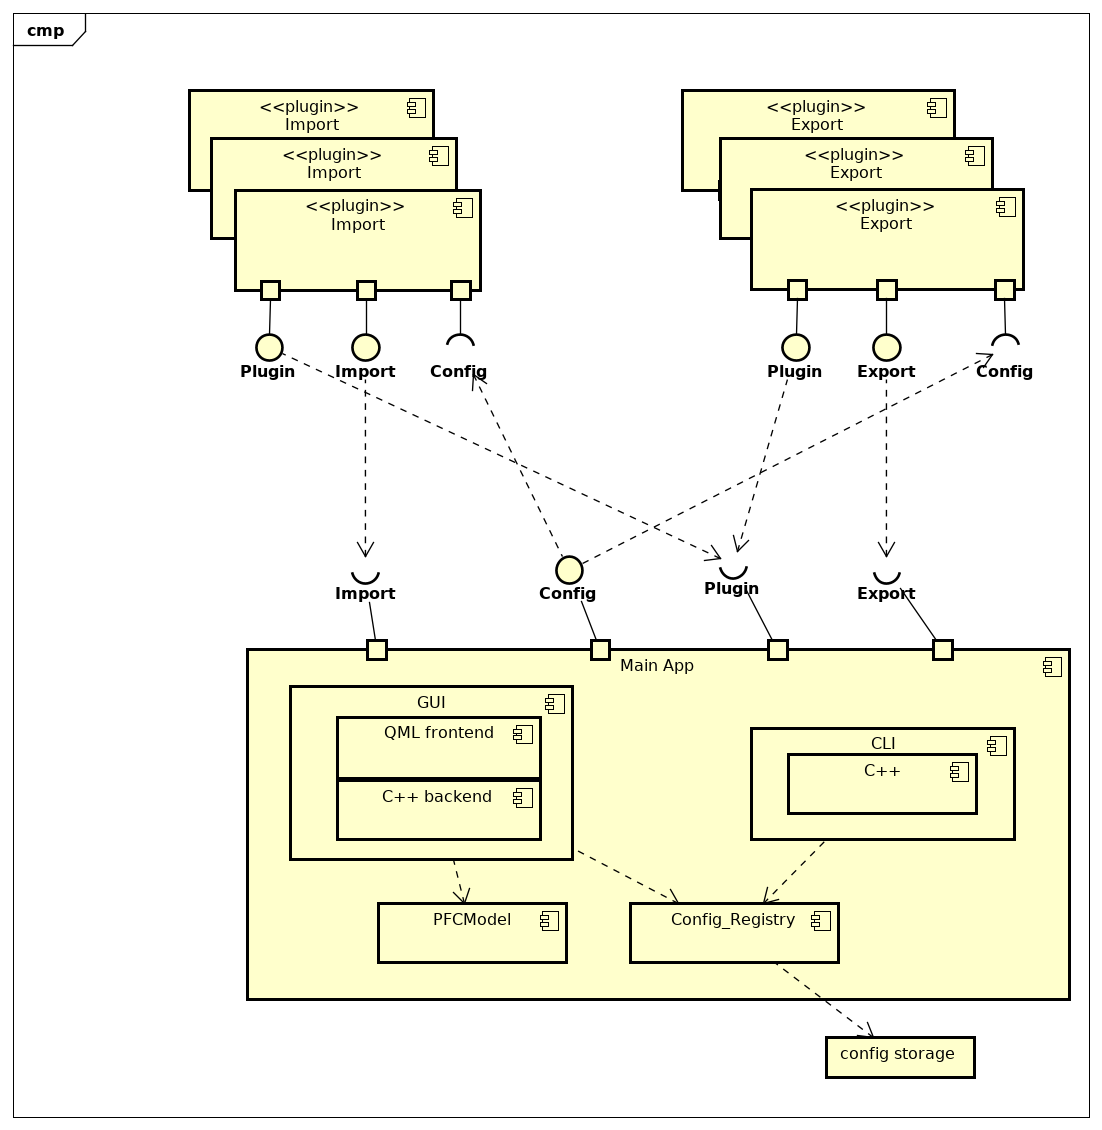
\includegraphics[width=\textwidth]{PluginArchitecture}
	\caption{Main application and plugin separation}
	\label{fig:comp}
\end{figure}
A plugin architecture as described in \ref{sec:resplug} was chosen for implementing \cmd{pfcrender}, as plugins to \cmd{pfcrender} will mainly consist of new Import/Export formats with limited intrinsic complexity and no dependencies on other plugins, avoiding aforementioned \textit{plugin hell} scenario.

The resulting component architecture is shown in figure \ref{fig:comp}. While the \gls{gui} could in theory be extracted to an export plugin as well, leaving the possibility to configure operation from the \gls{gui} was deemed useful. As this would depend on the \gls{gui} plugin receiving the QQuickItem config screen from the plugins, it would lead to dependencies among plugins, potentially leading to the \textit{plugin hell} situation described in \ref{sec:resplug}.

A key benefit of not binding the application to model import from the \gls{lsys} generator module is in extensibility. This architecture can also easily support a use-case, where a library of pre-iterated strings describing \gls{pfc}s is held in a different "PFC library tool" - e.g. categorized by their canonical names - like \textsc{Gosper's flowsnake} presented earlier - and can be easily integrated with the renderer by providing a new import plugin.

\chapter{Architecture Implementation}
\section{Application Configuration / Development Environment}

\subsection{Build System}
Travis CI / Codecov.io

Huge benefit to maintainability, clear insight on testing, fast feedback whether changes work.

Only feasible way to confirm multiplatform functionality without running 3 separate dev environments

They turned out to eat up about as much productivity in maintenance as they freed

Travis CI runs on Ubuntu 12.04LTS which reached End-of-Life in 2017. Ubuntu 14.04LTS support is still experimental, but even with the updated OS, the available tools are heavily outdated.

Standard gcc is a v4 with no support for C++11
Manually updating tools had ramifications as gcov was now ouptutting coverage data from gcov-5, lcov was using the old gcov-4 leading to no coverage being reported. Manually setting the gcov tool path resolved this issue, which - along with the time spent identifying the problem - was a significant time drain.

Still, the great benefit of this tool is that once it has been set up, it "just works" - running alongside the projects dev flow unintrusively and gives good insight into areas of improvement.

\section{Application configuration}

\section{Plugin Interface abstraction}
\subsubsection{Inheritance in Qt}
Implementing interfaces that are supposed to be used with Qt's meta object system is a slightly awkward procedure, as Qt's macros used to notify the moc about interface definitions and implementations are not namespace aware. 

This limitation pertains to interfaces exposing functionality from the Qt MetaObject system like signals/slots.

\section{Curve Creation}

\section{Graphical Output}
\subsection{Rendering the Model Curve}
While a PFC can be constructed segment by segment, the final size and position of the curve is not known until after the full curve is constructed.

The smallest rectangle fitting around a curve rendering is called its  \gls{bounding box}

Since the extent is not known beforehand, the resulting drawing must be transformed in such a way as to fit the given drawing device (screen, bitmap).

The resulting transformation can be done with a translation and scaling of the bounding box.

A performance-optimal way of calculating the bounding box is picking up minimum and maximum coordinates alongside the drawing avoiding a second parsing run of the model string.

Since the \gls{QPainter} API used by Qt is iterative in nature (\gls{QPainter} API), the transformation must be set before drawing begins. Setting a transformation only affect future drawing calls.

Using \gls{QPainter} thus forces precomputing of the bounding box.


\section{SVG Output}
\label{sec:svg}

\section{PDF Output}
\label{sec:pdf}

\section{Challenges faced during Implementation}

\subsection{Custom Geometry dunt werk liek it should}

\chapter{Application Performance}

\section{Problems}
\subsection{Model Creation}

\subsubsection{QQuickItem + Custom Geometry vs QQuickPaintedItem}
While QQuickPaintedItem allows us to use the QPainter API to generate the model for viewing, which is great, since it is also used by the SVG and PDF exporters, it is also painfully slow, as running callgrind on two parallel implementations shows.
do\_paint, which renders using QPainter API is a factor of 10 slower than manual creation of the OpenGL Vertex/Colordata

IMAGE : Callgrind cost

For this reason, a parallel implementation of both approaches was selected, with the GUI using rendering directly, and Painter based exporters using the QPainter API.

While this means that the GUI viewmodel can not be reused and the curve has to be rebuilt using qpainter on export, the GUI becomes responsive more quickly / scales to more iterates. As far as UX goes, the user can wait for file export, but not for an interactive GUI.
Especially since export is threadable/backgroundable.

\subsubsection{Encapsulation of Functionality (OOP) vs. Method Call overhead}
A lot of the OOP functionalites C++ offers, come at a performance cost.
While some of those classically named ones like stl containers are almost equivalent to plain C data, there are still very costly abstractions present in C++ wwhich can slow down a program significantly.
The gaming world programs C++ without exceptions for this exact reason (TODO: Reference), while those don't come into play here, method call overhead does.


\subsubsection{Runtime Optimization}
When optimizing a program for performance, it is essential to know where in the code the program spends the most time during typical execution, as optimizing 80\% of usecases by 20\% will be much more noticeable by users than speeding up 20\% of usecases by 80\% and is thus a better target for engineering effort.

While measuring the overall execution time of a program is as simple as starting and stopping a timer, looking for timings inside of executable, i.e. at the function level, needs additional instrumentation of the code that is executing. Tools that provide this instrumentation are called application profilers.

%TODO: WHAT DO PROFILERS DO EXACTLY?

One such tool - callgrind - is part of the valgrind analysis suite and well integrated into QtCreator.

\subsubsection{Compiler Optimizations and Inlining}
%TODO: Define stack frame
If a method is simple, but executes a billion times, the cycles spent saving and restoring stack frames while jumping between functions will make up a significant portion of the execution time of the program.

This is where so called inlining can help improve the runtime performance - as with all optimizations - at a cost. The tradeoff in this case being executable size.

Inlining a function means copying the content of its body to the place where it is executed. This skips stack frame saving and a jump/return instruction pair, but (TODO: show assembler of inlined for-loop) leads to the function body being duplicated, i.e. increasing code size with each execution.

While compilers do this type of optimization automatically, a keyword inline exists, that serves as a compiler hint and actually makes gcc/clang more likely to inline a function. Care has to be taken though, since inline has a different meaning when used on a function declaration. (in this case setting the function's definition as local to this translation unit, i.e. other TUs that include the header need to provide their own, identical function definition.

Since - contrary to embedded systems - program space and RAM are usually not a bottleneck on desktop systems, it often makes sense to optimize a program for runtime performance and ignore the larger executable size.

Modern compilers are able to optimize a program by several methods automatically, a user just needs to tell them how much of a tradeoff he is willing to take. The configuration (e.g. on GCC) for this feature is a commandline switch called optimization level. This can be -OS (optimize for size), nothing or -O0 (dont optimize) or -O1 through -O3, optimizing for performance with increasing aggressiveness / tolerance for increses in codesize.

The standard mode for release software is -O2.

\subsubsection{Link-Time Optimization}
Compilers can only optimize on the code they know, i.e. the code in the current translation unit.

Some optimizations (TODO: Which) only become possible when the full program is known, which is link-time. LTO is thus also known as full-program-optimization.

Insead of optimizing on a TU base, it optimizes llvm bytecode (TODO: llvm erkären?)

-flto=full


\subsubsection{Polymorphism and Performance}
Polymorphic classes are a key abstraction of C++ and are distinct from simple inheritance by the presence of the virtual keyword on at least some of their members.

This keyword enables a derived class, referred to through a pointer to the base class to execute its own implementation (a so called override) of the virtual member instead of the one (possibly, but not necessarily) implemented by the base class.

While this mechanism is fundamental to enabling C++ to provide the so called interface abstraction (TODO:Define), it comes with a performance cost.

Calls to a virtual function are not made by directly accessing the address of the callee, but access the so-called vtable instead. which is tasked with resolving the address of the member function.

This introduces several additional cycles (TODO: Measure how many or find in literature), which can become a significant bottleneck for performance, when the virtual function is called often, e.g. in our case, when parsing a character of the model string.


\chapter{Summary}
\label{cha:Summary}

The main driver in the decision to use the Qt framework was the decision to introduce a plugin architecture, because of the QLibrary abstraction they offer. Qt is not the most lightweight framework though, so if runtime extensibility is sacrificed, it would be possible to go with one of the much leaner frameworks like \ref{sfml} or \ref{cairo}, and possibly gain application performance.

\section{Followups}
\label{sec:Followups}
A followup on this thesis could be integration of model rendering to a OpenGL framebuffer object using a 3rd-party graphics library (e.g. \ref{cairo} or \ref{sdl}) and rendering that as a QQuickFramebufferObject\furl{http://doc.qt.io/qt-5/qquickframebufferobject.html} - thus evaluating performance of more drawing engines than the Qt-native QPainter.



% Literaturverzeichnis ---------------------------------------------------------
%   Das Literaturverzeichnis wird aus der BibTeX-Datenbank "Bibliographie.bib"
%   erstellt.
% ------------------------------------------------------------------------------
\bibliography{Bibliography} % Aufruf: bibtex Masterarbeit
\bibliographystyle{abbrvnat} % DIN-Stil des Literaturverzeichnisses

% Anhang -----------------------------------------------------------------------
%   Die Inhalte des Anhangs werden analog zu den Kapiteln inkludiert.
%   Dies geschieht in der Datei "Anhang.tex".
% ------------------------------------------------------------------------------
\begin{appendix}
    \clearpage
    \pagenumbering{roman}
    \chapter{Appendix}
    \label{sec:Appendix}
    % Rand der Aufzählungen in Tabellen anpassen
    \setdefaultleftmargin{1em}{}{}{}{}{}
    \nomenclature{API}{Application Programming Interface}
\nomenclature{ARIS}{Architektur integrierter Informationssysteme}
\nomenclature{BPR}{Business Process Reengineering}
\nomenclature{eEPK}{erweiterte Ereignisgesteuerte Prozesskette}
\nomenclature{EPK}{Ereignisgesteuerte Prozesskette}
\nomenclature{JMS}{Java Message Service}
\nomenclature{SDK}{Software Development Kit}
\nomenclature{URI}{Uniform Resource Identifier}
\nomenclature{URL}{Uniform Resource Locator}
\nomenclature{URN}{Uniform Resource Name}
\nomenclature{W3C}{World Wide Web Consortium}
\nomenclature{XML}{Extensible Markup Language}
\nomenclature{XPath}{XML Path Language}
\nomenclature{XSL}{Extensible Stylesheet Language}
\nomenclature{XSLT}{XSL Transformations}

\end{appendix}

% Index ------------------------------------------------------------------------
%   Zum Erstellen eines Index, die folgende Zeile auskommentieren.
% ------------------------------------------------------------------------------
\printindex

\end{document}
